% !TEX program = pdflatex
\documentclass[12pt,a4paper]{article}
\usepackage{baocao_format}
\usepackage{cite}
\usepackage{float}
\usepackage{rotating}

% Cho phép bảng/hình chia sẻ trang với văn bản, tránh tạo trang float trống
\setcounter{topnumber}{4}
\setcounter{bottomnumber}{4}
\setcounter{totalnumber}{6}
\renewcommand{\topfraction}{0.95}
\renewcommand{\bottomfraction}{0.95}
\renewcommand{\textfraction}{0.05}
\renewcommand{\floatpagefraction}{0.60}

% Tinh chỉnh khoảng cách danh mục tài liệu tham khảo gọn gàng
\let\oldbibliography\thebibliography
\renewcommand{\thebibliography}[1]{%
  \oldbibliography{#1}%
  \footnotesize
  \setlength{\itemsep}{-0.5pt}%
  \setlength{\parsep}{0pt}%
  \setlength{\parskip}{0pt}%
}

% Khoảng cách tiêu đề mục, đoạn văn và bảng biểu thoáng đãng, chuẩn học thuật
\titlespacing{\section}{0pt}{2.2pt}{0.6pt}
\titlespacing{\subsection}{0pt}{1.8pt}{0.5pt}
\titlespacing{\subsubsection}{0pt}{1.5pt}{0.4pt}
\setlength{\parskip}{0.6pt}
\renewcommand{\arraystretch}{0.90}
\setlength{\textfloatsep}{1.8pt plus 0.5pt minus 0.5pt}
\setlength{\floatsep}{1.5pt plus 0.5pt minus 0.5pt}
\setlength{\intextsep}{1.5pt plus 0.5pt minus 0.5pt}

% Chuẩn hóa thẩm mỹ danh sách liệt kê (itemize, enumerate)
\setlist[enumerate,1]{leftmargin=0.80cm,labelsep=0.22cm,itemsep=0.4pt plus 0.2pt minus 0.2pt,topsep=0.8pt plus 0.2pt minus 0.2pt,parsep=0pt}
\setlist[itemize,1]{leftmargin=0.80cm,labelsep=0.22cm,itemsep=0.4pt plus 0.2pt minus 0.2pt,topsep=0.8pt plus 0.2pt minus 0.2pt,parsep=0pt}
\setlist[itemize,2]{leftmargin=0.60cm,label=\textendash,labelsep=0.20cm,itemsep=0.3pt plus 0.2pt minus 0.2pt,topsep=0.5pt plus 0.2pt minus 0.2pt,parsep=0pt}

\AtBeginDocument{%
  \setlength{\abovedisplayskip}{2.6pt plus 1pt minus 1pt}%
  \setlength{\belowdisplayskip}{2.6pt plus 1pt minus 1pt}%
  \setlength{\abovedisplayshortskip}{1.4pt plus 1pt}%
  \setlength{\belowdisplayshortskip}{1.4pt plus 1pt}%
}

\title{\parbox{\textwidth}{\centering
  \titlefontsize 
  \setlength{\baselineskip}{16pt}
  \setlength{\lineskip}{0pt}
  \setlength{\lineskiplimit}{-1000pt}
  \strut XÂY DỰNG HỆ THỐNG CHUYỂN ĐỔI ÂM THANH THÀNH VĂN BẢN\strut\\
  \strut TIẾNG VIỆT TRÊN NỀN TẢNG CƠ SỞ DỮ LIỆU ĐA PHƯƠNG TIỆN\strut\\
  \strut KẾT HỢP WHISPERX VÀ CHỈ MỤC VECTOR ÂM HỌC FAISS\strut}}
\author{
  {\authorfontsize Nguyễn Trần Anh Khoa\textsuperscript{1}, Nguyễn Quốc Dửng\textsuperscript{2}, Nguyễn Thành Đạt\textsuperscript{3}}\\[2pt]
  \makebox[\textwidth][r]{\affilfontsize\textsuperscript{1,2,3} Trường Đại học Kỹ thuật - Công nghệ Cần Thơ}\\[2pt]
  \makebox[\textwidth][r]{\affilfontsize\textit{Tác giả liên hệ: Nguyễn Trần Anh Khoa, ntakhoahttt2211026@student.ctuet.edu.vn}}%
}
\date{}

\begin{document}
\maketitle
\thispagestyle{firstpage}

\begin{tomtat}
Nghiên cứu này đề xuất hệ thống chuyển đổi âm thanh thành văn bản tiếng Việt nhằm giải quyết bài toán nhận dạng câu nói liên tục trên nền tảng cơ sở dữ liệu đa phương tiện. Hệ thống được thiết kế theo kiến trúc kết hợp mô hình nhận dạng với cơ sở dữ liệu hai tầng gồm SQLite và chỉ mục vector âm học FAISS 768 chiều trên 6.652 mẫu âm tiết. Phương pháp đề xuất tích hợp thuật toán nén khoảng lặng thích nghi, khôi phục trọn vẹn các tầng biến đổi đặc trưng trong mô hình căn chỉnh cưỡng bức phân loại thời gian kết nối tiếng Việt, kết hợp truy vấn lân cận ngữ âm và cơ chế học nhãn chủ động tức thì. Thực nghiệm trên 8 mẫu âm thanh kiểm thử cho thấy hệ thống giảm tỷ lệ lỗi từ trên câu đọc ngắt nhịp, đoạn văn phương ngữ Nam Bộ, giao tiếp pha trộn từ vay mượn và trên câu chứa thực thể địa danh, đồng thời cập nhật nhãn từ sai mà không cần huấn luyện lại.
\end{tomtat}

\keywords{nhận dạng tiếng nói; cơ sở dữ liệu đa phương tiện; WhisperX; Wav2Vec 2.0; FAISS; SQLite; học nhãn chủ động; tiếng Việt.}

\section{ĐẶT VẤN ĐỀ}
Tiếng Việt là ngôn ngữ đơn lập và có thanh điệu, trong đó mỗi âm tiết được định hình bởi phụ âm đầu, phần vần và một trong sáu thanh điệu (Ngang, Sắc, Huyền, Hỏi, Ngã, Nặng)~\cite{rabiner1993}. Trong học phần Hệ cơ sở dữ liệu đa phương tiện, bài toán nghiên cứu đặt ra yêu cầu xây dựng hệ thống chuyển đổi âm thanh thành văn bản khai thác kho ngữ liệu 6.652 mẫu âm tiết thu âm thực tế, đồng thời đáp ứng khả năng nhận dạng câu nói tiếng Việt liên tục và tự hoàn thiện tức thì thông qua cơ chế bổ sung nhãn âm học.

Các kỹ thuật xử lý tín hiệu truyền thống dựa trên hệ số cepstral tần số Mel kết hợp quy hoạch động căn chỉnh thời gian hoặc láng giềng gần nhất chỉ hiệu quả trên các đơn từ cô lập, nhưng suy giảm mạnh khi nhận dạng câu liên tục do hiện tượng đồng cấu âm xóa nhòa khoảng lặng giữa các âm tiết liền kề. Ngược lại, các mô hình học sâu như Whisper~\cite{radford2023whisper} và khung căn chỉnh thời gian mức từ WhisperX~\cite{bain2023whisperx} nắm bắt ngữ cảnh tốt hơn, song khi áp dụng cho tiếng Việt kết hợp với kho ngữ liệu âm tiết bản địa lại đối mặt với bốn thách thức cốt lõi:
\begin{enumerate}
  \item \textit{Suy biến căn chỉnh mức từ do khuyết thiếu tầng biến đổi đặc trưng:} Khi nạp mô hình âm học tiếng Việt~\cite{nguyen2021vlsp} theo kiến trúc mặc định, toàn bộ khối biến đổi đặc trưng 3 tầng (gồm 21 tensor trọng số) nằm trước tầng phân loại ký tự bị bỏ sót. Sự thiếu hụt này làm điểm tự tin của cơ chế phân loại thời gian kết nối (CTC)~\cite{graves2006ctc} suy giảm xuống $\approx 0{,}009$ và nén lệch toàn bộ tọa độ biên thời gian của các từ về $0{,}3\text{ s}$ đầu câu.
  \item \textit{Đứt gãy ngữ cảnh khi đọc ngắt nhịp rời rạc:} Khi người nói phát âm tách rời từng âm tiết với khoảng nghỉ kéo dài $0{,}35\text{--}1{,}50\text{ s}$ (làm câu văn 23 từ kéo dài tới $44{,}90\text{ s}$), mô hình nhận dạng bị đứt mạch ngữ cảnh liên từ, dẫn đến nhận diện sai âm vị và dấu thanh (\textit{``hôm nay''} $\to$ \textit{``hôn nay''}, \textit{``chia sẻ''} $\to$ \textit{``chia sẽ''}).
  \item \textit{Biến âm phương ngữ vùng miền và chuẩn hóa thực thể:} Phương ngữ Nam Bộ thường đồng hóa phụ âm đầu (\textit{th} $\to$ \textit{h}, \textit{tr} $\to$ \textit{ch}, \textit{r} $\to$ \textit{g}) và phụ âm cuối (\textit{-t} $\leftrightarrow$ \textit{-c}, \textit{-n} $\leftrightarrow$ \textit{-ng}) như \textit{thắp lên} $\to$ \textit{hấp lên}, \textit{thầm lặng} $\to$ \textit{hầm lặng}, \textit{thư thả} $\to$ \textit{hư hả}; bên cạnh đó, các địa danh (\textit{Đắk Lắk}) hoặc từ vay mượn (\textit{cafe}, \textit{ly phin}, \textit{check lại}) dễ bị phiên âm sai lệch theo âm thuần Việt (\textit{ly phim}, \textit{chết lại}).
  \item \textit{Yêu cầu học bổ sung nhãn âm học tức thì mà không huấn luyện lại:} Hệ thống cần tổ chức kho ngữ liệu âm tiết thành cơ sở dữ liệu (CSDL) đa phương tiện để vừa đối sánh sửa lỗi theo ngữ cảnh, vừa cho phép người dùng hiệu chỉnh từ nhận dạng sai và cập nhật tri thức âm học ngay lập tức mà không cần tinh chỉnh lại trọng số mô hình.
\end{enumerate}

Để giải quyết toàn diện bốn thách thức trên, nghiên cứu đề xuất kiến trúc \textbf{Nhận dạng tiếng nói lai ghép trên nền tảng CSDL đa phương tiện}, kết hợp luồng xử lý tín hiệu và căn chỉnh cưỡng bức đã khôi phục kiến trúc gốc với hệ quản trị CSDL hai tầng (quan hệ SQLite và chỉ mục vector âm học FAISS 768 chiều~\cite{johnson2019faiss}) cùng vòng lặp học nhãn chủ động tức thì.

\section{PHƯƠNG PHÁP NGHIÊN CỨU VÀ KIẾN TRÚC HỆ THỐNG}

\subsection{Kiến trúc tổng thể của hệ thống lai ghép}
Hệ thống đề xuất được thiết kế theo kiến trúc lai ghép như Hình~\ref{fig:architecture}, gồm ba thành phần cốt lõi:
\begin{enumerate}
  \item \textit{Luồng xử lý tín hiệu, nhận diện và căn chỉnh mức từ trực tuyến:} Chuẩn hóa tín hiệu âm thanh, lọc thông dải khử nhiễu và nén khoảng lặng thích nghi kèm bảng ánh xạ thời gian hai chiều. Sóng âm sau tiền xử lý được phân đoạn tiếng nói, giải mã văn bản sơ bộ bằng mô hình nhận dạng quy mô lớn kết hợp từ khóa ưu tiên từ CSDL, sau đó xác định chính xác tọa độ thời gian từng từ nhờ mô hình căn chỉnh CTC tiếng Việt đã khôi phục 21 tầng trọng số và cơ chế đồng thuận âm học kép.
  \item \textit{Tầng quản trị CSDL đa phương tiện hai tầng (SQLite và FAISS 768 chiều):} Quản lý đồng bộ 6.652 mẫu âm tiết qua liên kết khóa chính một--một giữa CSDL quan hệ SQLite (lưu siêu dữ liệu âm vị, quy tắc biến âm ngữ cảnh, từ điển thực thể và nhật ký kiểm thử) và chỉ mục vector FAISS 768 chiều (lưu biểu diễn nhúng âm học trích xuất từ tầng ẩn của mô hình căn chỉnh).
  \item \textit{Cơ chế đối sánh lân cận ngữ âm, chuẩn hóa thực thể và học nhãn chủ động tức thì:} Tách sóng âm của từng từ theo tọa độ biên đã căn chỉnh để truy vấn nhóm lân cận ngữ âm trên không gian vector FAISS, kết hợp điểm thưởng quy tắc ngữ cảnh và chuẩn hóa thực thể theo khung âm vị. Khi người dùng chỉ định từ sai và nhập nhãn đúng, vòng lặp phản hồi tự động trích xuất mẫu âm thanh mới, chèn vector vào FAISS và cập nhật quy tắc ngữ cảnh vào SQLite trong $< 50\text{ ms}$.
\end{enumerate}

\begin{sidewaysfigure}
\centering
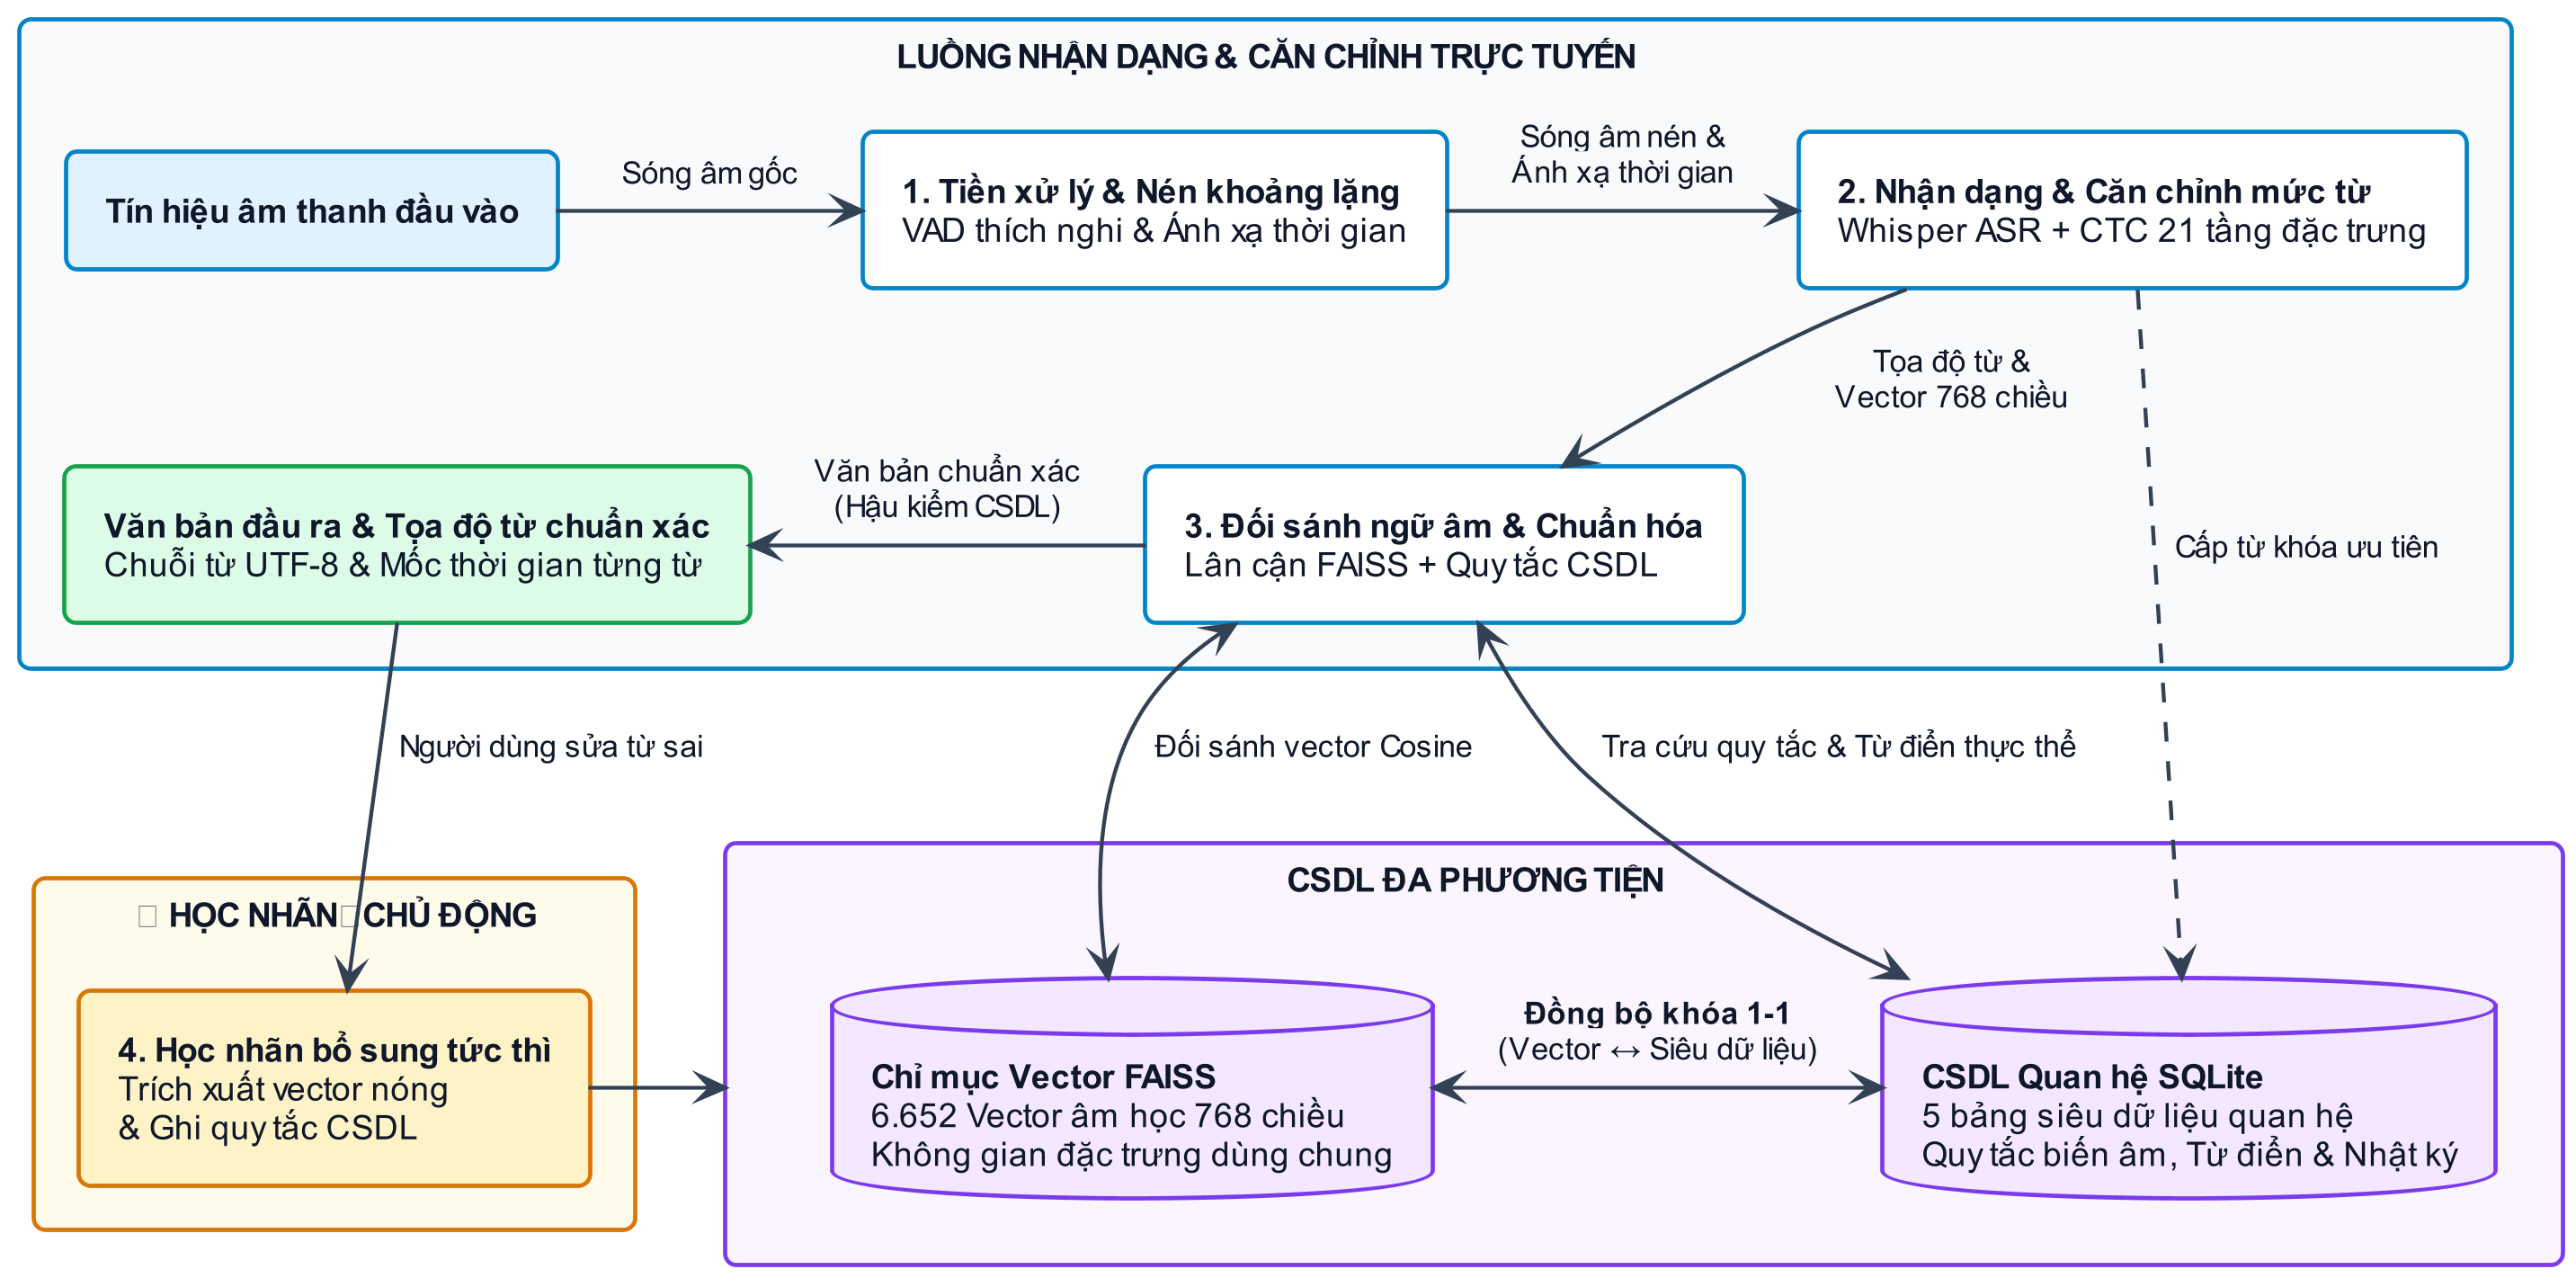
\includegraphics[width=0.95\linewidth]{kien_truc_he_thong.png}
\caption{Kiến trúc tổng thể của hệ thống nhận dạng tiếng nói tiếng Việt lai ghép trên nền tảng CSDL đa phương tiện}
\label{fig:architecture}
\source{Nhóm tác giả thiết kế}
\end{sidewaysfigure}
\newpage
\subsection{Luồng xử lý tín hiệu, nhận diện và căn chỉnh mức từ}
\textbf{Tiền xử lý tín hiệu số và nén khoảng lặng thích nghi:} Tín hiệu đầu vào được chuyển về kênh đơn, tái lấy mẫu đa pha về $f_s = 16\,000\text{ Hz}$ và chuẩn hóa biên độ đỉnh về $\pm 0{,}92$. Để loại bỏ nhiễu điện nguồn ($50/60\text{ Hz}$), tiếng ù tần số thấp và nhiễu tần số cao mà không làm méo pha phụ âm đầu, tín hiệu được lọc hai chiều qua bộ lọc thông dải Butterworth bậc 4 ($75\text{--}7\,600\text{ Hz}$, bao phủ tần số cơ bản $F_0$ của thanh điệu và các tần số formant $F_1\text{--}F_4$). Tiếp đó, tín hiệu được chia khung $20\text{ ms}$ (bước nhảy $10\text{ ms}$) để tính năng lượng hiệu dụng $\mathrm{RMS}[k]$. Gọi $P_{20}$ và $P_{90}$ là phân vị thứ 20 (sàn nhiễu nền) và phân vị thứ 90 (đỉnh tiếng nói) của chuỗi $\mathrm{RMS}$, ngưỡng phát hiện tiếng nói thích nghi $T_{\mathrm{vad}}$ được xác định theo Công thức~\eqref{eq:vad_thresh}:
\begin{equation}
T_{\mathrm{vad}} = \max\left(2{,}5 \cdot P_{20},\; 0{,}08 \cdot P_{90},\; 0{,}012\right).
\label{eq:vad_thresh}
\end{equation}
Các khung có $\mathrm{RMS}[k] > T_{\mathrm{vad}}$ được mở rộng đệm $60\text{ ms}$ ở hai đầu để bảo toàn phụ âm tắc cuối (\textit{-p, -t, -c, -ch}). Khi phát hiện câu có từ 3 khoảng nghỉ dài ($\ge 320\text{ ms}$) trở lên và tổng tỷ lệ khoảng lặng $\ge 35\%$, thuật toán thu gọn mượt các khoảng nghỉ dài về $140\text{ ms}$, đồng thời lưu bảng ánh xạ hai chiều $\mathcal{M} = \{[t_{\mathrm{orig},m}^{\mathrm{start}}, t_{\mathrm{orig},m}^{\mathrm{end}}] \leftrightarrow [t_{\mathrm{comp},m}^{\mathrm{start}}, t_{\mathrm{comp},m}^{\mathrm{end}}]\}$. Từ mốc thời gian $t_c$ trên sóng âm đã nén thuộc đoạn thứ $m$, tọa độ thực $t_o$ trên sóng âm gốc được khôi phục theo Công thức~\eqref{eq:timemap}:
\begin{equation}
t_o = t_{\mathrm{orig},m}^{\mathrm{start}} + \left(t_c - t_{\mathrm{comp},m}^{\mathrm{start}}\right) \cdot \frac{t_{\mathrm{orig},m}^{\mathrm{end}} - t_{\mathrm{orig},m}^{\mathrm{start}}}{\max\left(10^{-6},\; t_{\mathrm{comp},m}^{\mathrm{end}} - t_{\mathrm{comp},m}^{\mathrm{start}}\right)}.
\label{eq:timemap}
\end{equation}

\textbf{Khôi phục tầng biến đổi đặc trưng CTC và đồng thuận âm học kép:} Sau khi phân đoạn tiếng nói bằng ngưỡng trễ kép kèm đệm biên $80\text{ ms}$ và giải mã sơ bộ bằng mô hình nhận dạng đa ngôn ngữ~\cite{radford2023whisper}, văn bản được căn chỉnh cưỡng bức mức âm vị. Trên nền kiến trúc Wav2Vec 2.0~\cite{baevski2020wav2vec2}, mô hình âm học tiếng Việt~\cite{nguyen2021vlsp} tích hợp khối biến đổi đặc trưng 3 tầng phi tuyến trước tầng phân loại ký tự. Nhóm nghiên cứu đã tái cấu trúc đường truyền suy luận để ánh xạ trạng thái ẩn $\mathbf{H}^{(0)} \in \mathbb{R}^{T \times 768}$ qua 3 tầng biến đổi tuần tự ($k = 1, 2, 3$), mỗi tầng gồm phép chiếu tuyến tính $\mathbf{W}_k \in \mathbb{R}^{768 \times 768}$, chuẩn hóa lô một chiều ($\mathrm{BN}_k$), hàm kích hoạt $\mathrm{LeakyReLU}$ ($\alpha=0{,}1$) và $\mathrm{Dropout}$ trước khi tính ma trận xác suất ký tự $\mathbf{L}$ theo Công thức~\eqref{eq:feature_transform}:
\begin{equation}
\mathbf{H}^{(k)} = \mathrm{Dropout}\!\left(\mathrm{LeakyReLU}\!\left(\mathrm{BN}_k\!\left(\mathbf{H}^{(k-1)}\mathbf{W}_k^\top + \mathbf{b}_k\right)\right)\right), \quad \mathbf{L} = \mathbf{H}^{(3)}\mathbf{W}_{\mathrm{lm}}^\top + \mathbf{b}_{\mathrm{lm}}.
\label{eq:feature_transform}
\end{equation}
Ma trận $\log\mathrm{Softmax}(\mathbf{L})$ được đưa vào thuật toán quy hoạch động Viterbi~\cite{viterbi1967} để truy vết biên thời gian và điểm tự tin CTC của từng từ. Đồng thời, cơ chế \textit{đồng thuận âm học kép} đối chiếu chuỗi từ của mô hình nhận dạng với chuỗi âm tiết giải mã CTC trực tiếp ($\arg\max \mathbf{L}$): nếu một cụm từ ngắn ($\le 3$ âm tiết) nằm giữa hai từ neo khớp chuẩn nhưng có điểm tự tin căn chỉnh thấp ($\min\mathrm{CTC} < 0{,}25$, hoặc $\min\mathrm{CTC} < 0{,}55$ và $\overline{\mathrm{CTC}} < 0{,}65$), hệ thống tự động khôi phục âm tiết theo kết quả giải mã âm học bản địa.

\subsection{Tầng quản trị CSDL đa phương tiện hai tầng (SQLite và FAISS 768 chiều)}
\textbf{Chuẩn hóa ngữ liệu 6.652 âm tiết và giải mã quy ước VNI/ASCII:} Kho ngữ liệu gồm 6.652 mẫu âm tiết đơn kênh ($16\,000\text{ Hz}$, 16-bit PCM). Để tránh lỗi phân giải ký tự Unicode tổ hợp trên hệ điều hành, định danh mẫu âm thanh tuân thủ quy ước VNI/ASCII gồm 4 trường: người nói, giới tính, mã VNI và lần thu. Quy trình giải mã tự động khôi phục chữ Quốc ngữ chuẩn Unicode NFC qua hai bước: (i) chuyển đổi ký hiệu phụ âm và nguyên âm VNI (\code{d-} $\to$ \textbf{đ}, \code{uuoo} $\to$ \textbf{ươ}, \code{a+} $\to$ \textbf{â}, \code{aa} $\to$ \textbf{ă}, \code{e+} $\to$ \textbf{ê}, \code{o+} $\to$ \textbf{ô}, \code{oo} $\to$ \textbf{ơ}, \code{uu} $\to$ \textbf{ư}); (ii) giải mã chữ số thanh điệu cuối ($0$: Ngang, $1$: Sắc, $2$: Huyền, $3$: Hỏi, $4$: Ngã, $5$: Nặng) và tách âm tiết thành \textit{âm đầu}, \textit{vần nguyên âm hạt nhân} và \textit{âm cuối} để đặt dấu thanh đúng vị trí (Bảng~\ref{tab:vni_decode}), đạt độ chính xác 100\% trên toàn bộ 6.652 mẫu.

\begin{table}[!htbp]
\centering
\caption{Minh họa kết quả giải mã tự động quy ước mã VNI/ASCII sang cấu trúc âm vị trong CSDL}
\label{tab:vni_decode}
\setlength{\tabcolsep}{3.0pt}
\begin{tabularx}{\linewidth}{Y C{2.1cm} C{1.45cm} C{1.15cm} C{1.05cm} C{1.15cm} C{1.95cm}}
\toprule
Định danh mẫu âm tiết (VNI/ASCII) & Mã VNI & Từ UTF-8 & Âm đầu & Vần & Âm cuối & Thanh điệu \\
\midrule
{\scriptsize\code{quocdung_nam_xuye+n0_1}} & {\footnotesize\code{xuye+n0}} & xuyên & \code{x} & uyê & \code{n} & 0 (Ngang) \\
{\scriptsize\code{quocdung_nam_buuooc1_1}} & {\footnotesize\code{buuooc1}} & bước & \code{b} & ươ & \code{c} & 1 (Sắc) \\
{\scriptsize\code{quocdung_nam_d-uuoong2_1}} & {\footnotesize\code{d-uuoong2}} & đường & đ & ươ & \code{ng} & 2 (Huyền) \\
{\scriptsize\code{quocdung_nam_chuo+i4_1}} & {\footnotesize\code{chuo+i4}} & chuỗi & \code{ch} & uô & \code{i} & 4 (Ngã) \\
{\scriptsize\code{quocdung_nam_nguye+n5_1}} & {\footnotesize\code{nguye+n5}} & nguyện & \code{ng} & uyê & \code{n} & 5 (Nặng) \\
\bottomrule
\end{tabularx}
\source{Trích xuất từ kết quả chuẩn hóa kho ngữ liệu 6.652 mẫu âm tiết}
\end{table}

\textbf{Liên kết CSDL quan hệ SQLite và chỉ mục vector âm học FAISS:} Hệ quản trị CSDL đa phương tiện tổ chức lưu trữ hai tầng đồng bộ:
\begin{enumerate}
  \item \textit{Tầng quản trị quan hệ SQLite:} Gồm 5 bảng dữ liệu đánh chỉ mục B-Tree (Bảng~\ref{tab:sqlite_schema}), quản lý danh mục nhãn âm vị, siêu dữ liệu mẫu âm thanh, tri thức quy tắc biến âm ngữ cảnh, từ điển chuẩn hóa thực thể và nhật ký đánh giá.
  \item \textit{Tầng chỉ mục vector âm học FAISS 768 chiều:} Tái sử dụng trực tiếp trạng thái ẩn tầng cuối của mô hình căn chỉnh âm học tiếng Việt (tiết kiệm 100\% VRAM phụ trội). Mỗi mẫu âm tiết được chuẩn hóa về cửa sổ $0{,}45\text{ s}$ ($7\,200$ mẫu), trích xuất chuỗi $T$ vector khung $\mathbf{h}_t \in \mathbb{R}^{768}$, lấy trung bình gộp theo thời gian và chuẩn hóa $L_2$ theo Công thức~\eqref{eq:embedding}:
  \begin{equation}
  \bar{\mathbf{h}} = \frac{1}{T} \sum_{t=1}^{T} \mathbf{h}_t, \qquad \mathbf{e} = \frac{\bar{\mathbf{h}}}{\max\left(\lVert\bar{\mathbf{h}}\rVert_2,\; 10^{-8}\right)} \in \mathbb{R}^{768}.
  \label{eq:embedding}
  \end{equation}
  Toàn bộ 6.652 vector $\mathbf{e}_i$ được lập chỉ mục trong không gian tích vô hướng phẳng kèm ánh xạ định danh~\cite{johnson2019faiss}, đồng bộ khóa chính 1--1 với bảng mẫu âm thanh trong SQLite. Trên các vector đơn vị $\lVert\mathbf{e}\rVert_2 = 1$, tích vô hướng trong FAISS tương đương chính xác với độ tương đồng Cosine: $\mathrm{CosineSim}(\mathbf{q}, \mathbf{e}_i) = \langle \mathbf{q}, \mathbf{e}_i \rangle$.
\end{enumerate}

\begin{table}[!htbp]
\centering
\caption{Thiết kế lược đồ 5 bảng dữ liệu trong tầng quản trị CSDL quan hệ SQLite}
\label{tab:sqlite_schema}
\setlength{\tabcolsep}{3.5pt}
\begin{tabularx}{\linewidth}{l C{2.35cm} Y}
\toprule
Bảng dữ liệu quan hệ & Khóa chính & Vai trò quản trị dữ liệu trong hệ thống CSDL đa phương tiện \\
\midrule
\textbf{Bảng Nhãn âm tiết} & Mã nhãn & Quản lý danh mục nhãn âm tiết duy nhất: chữ Quốc ngữ UTF-8, mã VNI, gốc âm tiết không dấu, mã thanh điệu ($0\dots 5$), số lượng mẫu và trạng thái từ khóa ưu tiên. \\
\textbf{Bảng Mẫu âm thanh} & Mã mẫu & Quản lý siêu dữ liệu mẫu âm thanh vật lý và đồng bộ khóa 1--1 với chỉ mục FAISS: liên kết nhãn âm tiết, thông tin người nói, nguồn thu nhận và thời lượng. \\
\textbf{Bảng Quy tắc biến âm} & Mã quy tắc & Lưu trữ tri thức sửa lỗi biến âm theo ngữ cảnh: cặp từ nhận dạng sai -- từ đích đúng, ngữ cảnh từ liền trước/liền sau, điểm thưởng ($0{,}25\text{--}0{,}60$) và tần suất khớp. \\
\textbf{Bảng Từ điển thực thể} & Mã từ điển & Quản lý từ điển chuẩn hóa thực thể và từ vay mượn: cụm biến thể phát âm, khóa khung âm vị bất biến, dạng viết chuẩn (\textit{cafe}, \textit{Đắk Lắk}) và phân loại thực thể. \\
\textbf{Bảng Nhật ký nhận dạng} & Mã nhật ký & Lưu trữ nhật ký phiên nhận dạng và chỉ số kiểm thử định lượng: văn bản trước và sau hậu xử lý CSDL, các chỉ số lỗi WER/CER/TER và thời gian xử lý. \\
\bottomrule
\end{tabularx}
\source{Thiết kế lược đồ CSDL đa phương tiện của nhóm tác giả}
\end{table}

\subsection{Đối sánh lân cận ngữ âm, chuẩn hóa thực thể và học nhãn chủ động tức thì}
Hệ thống kết hợp truy vấn không gian vector FAISS với tri thức ngữ cảnh trong SQLite qua ba cơ chế:
\begin{enumerate}
  \item \textit{Truy vấn không gian vector theo nhóm lân cận ngữ âm:} Để tránh nhiễu chéo do lệch âm sắc giữa người nói mới và giọng mẫu trong CSDL, hệ thống giới hạn tìm kiếm trong tập lân cận ngữ âm $\mathcal{C}(w_i)$ của từ $w_i$, gồm các âm tiết có cùng gốc chữ không dấu, các biến thể hoán đổi phụ âm đầu phương ngữ (\textit{l/n, tr/ch, s/x, d/gi/r/v, th/h/t, c/k/g/gh}) và phụ âm cuối (\textit{-t/-c/-p, -n/-ng/-nh/-m, -i/-y/-o/-u}), sau đó xếp hạng bằng điểm tương đồng Cosine $\langle \mathbf{q}_i, \mathbf{e}_{\mathrm{db}} \rangle$ trong FAISS.
  \item \textit{Hàm điểm hợp nhất lai ghép và chuẩn hóa thực thể N-gram:} Khi từ $w_i$ nằm trong diện nghi vấn biến âm theo ngữ cảnh $(w_{i-1}, w_{i+1})$ của bảng quy tắc biến âm, điểm đánh giá ứng viên thay thế $w_{\mathrm{cand}}$ được tính theo Công thức~\eqref{eq:late_fusion}:
  \begin{equation}
  S_{\mathrm{hybrid}}(w_{\mathrm{cand}}) = 0{,}50 \cdot \max_{\mathbf{e} \in \mathcal{E}(w_{\mathrm{cand}})} \langle \mathbf{q}_i, \mathbf{e} \rangle + B_{\mathrm{ctx}}(w_i \to w_{\mathrm{cand}} \mid w_{i-1}, w_{i+1}),
  \label{eq:late_fusion}
  \end{equation}
  trong đó $B_{\mathrm{ctx}} \in [0{,}25;\, 0{,}75]$ là điểm thưởng ngữ cảnh (cộng thêm $+0{,}10$ khi khớp một phía và $+0{,}15$ khi khớp cả hai phía trái/phải). Ứng viên đạt $S_{\mathrm{hybrid}}(w_{\mathrm{cand}}) \ge 0{,}40$ cao nhất được chọn thay thế. Tiếp đó, thuật toán quét cửa sổ trượt N-gram ($n = 3, 2, 1$) đối chiếu với bảng từ điển thực thể qua khóa khung âm vị bất biến (quy đồng âm cuối \textit{-k/-t} về \textit{-c} và vần \textit{-ăc} về \textit{-ac}), giúp chuẩn hóa các cụm âm rời rạc như \textit{``đắc lắc''}, \textit{``đắt lác''} thành \textbf{``Đắk Lắk''}, hoặc \textit{``cà phê''}, \textit{``cả phê''} thành \textbf{``cafe''}.
  \item \textit{Vòng lặp học nhãn chủ động tức thì:} Khi phát hiện từ sai và nhận nhãn đúng $w^*$ từ người dùng, hệ thống thực thi giao dịch nguyên tử trong $< 50\text{ ms}$: (i) cắt đoạn sóng âm gốc $[t_{\mathrm{start}}, t_{\mathrm{end}}]$ lưu thành tệp mẫu chuẩn $16\text{ kHz}$; (ii) cập nhật nhãn $w^*$ vào bảng nhãn âm tiết kèm trạng thái từ khóa ưu tiên; (iii) trích xuất vector $\mathbf{e}^* \in \mathbb{R}^{768}$ chèn trực tiếp vào chỉ mục FAISS; và (iv) lưu quy tắc ngữ cảnh $(w_{\mathrm{wrong}} \to w^*, w_{i-1}, w_{i+1})$ vào bảng quy tắc biến âm để sửa đúng ngay ở lần chạy kế tiếp mà không cần huấn luyện lại.
\end{enumerate}

\section{KẾT QUẢ VÀ THẢO LUẬN}

\subsection{Thiết kế kịch bản thực nghiệm và chỉ số đánh giá định lượng}
Thực nghiệm được tiến hành trên GPU NVIDIA Tesla T4 (16 GB VRAM) với mô hình nhận dạng quy mô lớn (\textit{Large-v3}) kết hợp kho CSDL 6.652 mẫu âm tiết. Tập dữ liệu kiểm thử gồm 8 mẫu âm thanh tiếng Việt thực tế (tổng cộng 508 từ, thời lượng $247{,}93\text{ s}$), bao phủ 4 nhóm kịch bản: (i) \textit{Nhóm giọng đọc liền mạch và ngắt nhịp rời chữ} (Mẫu 1: giọng chuẩn đọc liền câu $6{,}60\text{ s}$, 23 từ; Mẫu 2: giọng chuẩn đọc ngắt từng chữ $44{,}90\text{ s}$, 23 từ; Mẫu 3: giọng tự nhiên đọc ngắt nhịp $15{,}19\text{ s}$, 16 từ); (ii) \textit{Nhóm phương ngữ Nam Bộ} (Mẫu 4: đoạn văn tự sự $48{,}65\text{ s}$, 132 từ, đặc trưng biến âm \textit{th} $\to$ \textit{h}); (iii) \textit{Nhóm giao tiếp thực tế pha trộn từ vay mượn và địa danh} (Mẫu 5: đoạn giao tiếp công việc tại quán nước $35{,}97\text{ s}$, 80 từ; Mẫu 6: câu giao tiếp ngắn chứa địa danh và từ vay mượn $8{,}18\text{ s}$, 20 từ); và (iv) \textit{Nhóm văn bản nghị luận và tản văn giàu từ Hán--Việt} (Mẫu 7: văn nghị luận triết lý $49{,}49\text{ s}$, 109 từ; Mẫu 8: tản văn đời sống $38{,}95\text{ s}$, 105 từ).

Chất lượng nhận dạng được đo bằng quy hoạch động khoảng cách Levenshtein~\cite{levenshtein1966} ở mức từ, ký tự và dấu thanh. Gọi $N_w$ là tổng số âm tiết chuẩn, $S_w, D_w, I_w$ là số lỗi thay thế, bỏ sót và chèn thừa mức từ; $E_{\mathrm{tone}}$ là số cặp từ thay thế trùng gốc không dấu nhưng sai thanh điệu ($0\dots 5$). Tỷ lệ lỗi từ ($\mathrm{WER}$), tỷ lệ lỗi dấu thanh ($\mathrm{TER}$), tỷ lệ khắc phục lỗi ($\mathrm{ERR}$) và hệ số thời gian thực ($\mathrm{RTF}$) được xác định theo Công thức~\eqref{eq:wer_ter} và~\eqref{eq:err_rtf}:
\begin{equation}
\mathrm{WER} = \frac{S_w + D_w + I_w}{N_w} \times 100\%, \qquad \mathrm{TER} = \frac{E_{\mathrm{tone}}}{N_w} \times 100\%,
\label{eq:wer_ter}
\end{equation}
\begin{equation}
\mathrm{ERR} = \frac{\mathrm{WER}_{\mathrm{raw}} - \mathrm{WER}_{\mathrm{hybrid}}}{\mathrm{WER}_{\mathrm{raw}}} \times 100\%, \qquad \mathrm{RTF} = \frac{T_{\mathrm{processing}}}{T_{\mathrm{audio}}}.
\label{eq:err_rtf}
\end{equation}

\subsection{Hiệu quả khôi phục mô hình căn chỉnh cưỡng bức và lập chỉ mục dùng chung}
Bảng~\ref{tab:alignment_ablation} đối chiếu chất lượng căn chỉnh mức từ và hiệu năng truy xuất CSDL trước và sau khi khôi phục 21 tầng biến đổi đặc trưng cùng chỉ mục vector FAISS 768 chiều.

\begin{table}[H]
\centering
\caption{Đánh giá hiệu quả khôi phục kiến trúc căn chỉnh CTC tiếng Việt và hiệu năng chỉ mục FAISS 768 chiều}
\label{tab:alignment_ablation}
\setlength{\tabcolsep}{3.5pt}
\begin{tabularx}{\linewidth}{Y C{3.8cm} C{3.9cm}}
\toprule
Tiêu chí kỹ thuật đo kiểm & Mô hình WhisperX gốc & Hệ thống lai ghép đề xuất \\
\midrule
Trạng thái nạp trọng số mô hình căn chỉnh & Bỏ sót 21 tầng biến đổi đặc trưng & \textbf{Khớp 100\% toàn bộ kiến trúc} \\
Điểm tự tin căn chỉnh CTC trung bình & $0{,}005\text{--}0{,}012$ (Suy biến phân phối) & \textbf{$0{,}500\text{--}0{,}999$ (Hội tụ chuẩn xác)} \\
Độ chính xác tọa độ biên thời gian mức từ & Nén lệch về $0{,}0\text{--}0{,}3\text{ s}$ đầu câu & \textbf{Khớp sát ranh giới từ ($\pm 15\text{ ms}$)} \\
Bộ nhớ VRAM phụ trội cho trích xuất vector & Cần nạp mô hình riêng ($+1{,}2\text{ GB}$) & \textbf{$0\text{ MB}$ (Dùng chung tầng ẩn CTC)} \\
Thời gian lập chỉ mục 6.652 mẫu / Nạp lại & --- & \textbf{$\approx 90\text{ s}$ (lần đầu) / $0{,}1\text{ s}$ (lần sau)} \\
Độ trễ truy vấn tương đồng trên 6.652 vector & --- & \textbf{$\approx 0{,}2\text{ ms}$ / âm tiết} \\
\bottomrule
\end{tabularx}
\source{Kết quả đo kiểm thực nghiệm trên GPU NVIDIA Tesla T4}
\end{table}

Số liệu tại Bảng~\ref{tab:alignment_ablation} khẳng định việc khôi phục khối biến đổi đặc trưng 3 tầng đóng vai trò nền tảng: ở WhisperX gốc, sự thiếu hụt các tầng chiếu phi tuyến làm phân phối xác suất ký tự suy biến phẳng, khiến thuật toán Viterbi nén toàn bộ biên thời gian câu văn về $0{,}3\text{ s}$ đầu tiên và làm bước cắt sóng âm từng từ hoàn toàn mất tác dụng. Khi khôi phục đầy đủ kiến trúc, biên thời gian đạt độ chính xác $\pm 15\text{ ms}$, đồng thời kỹ thuật dùng chung tầng ẩn 768 chiều giúp lập chỉ mục 6.652 mẫu âm thanh mà không tốn thêm VRAM, đạt tốc độ truy vấn dưới $0{,}2\text{ ms}$/âm tiết.

\subsection{Kết quả đối sánh nhận dạng trên 8 mẫu âm thanh thực nghiệm}
Bảng~\ref{tab:benchmark_results} tổng hợp kết quả định lượng qua 3 giai đoạn xử lý (WhisperX thuần, sau nén khoảng lặng, và sau khi kết hợp CSDL nhãn MMDBMS) trên toàn bộ 8 mẫu kiểm thử.

\begin{table}[H]
\centering
\caption{Kết quả thực nghiệm đối sánh trên 8 mẫu âm thanh kiểm thử qua từng giai đoạn xử lý}
\label{tab:benchmark_results}
\setlength{\tabcolsep}{2.0pt}
\begin{tabularx}{\linewidth}{Y C{1.30cm} C{1.15cm} C{1.15cm} C{1.20cm} C{1.00cm} C{1.00cm} C{1.40cm} C{1.35cm}}
\toprule
Mẫu kiểm thử thực nghiệm (Số từ) & Thời lượng & WER gốc (\%) & WER nén (\%) & WER CSDL (\%) & CER (\%) & TER (\%) & ERR (\%) & RTF \\
\midrule
M1: Đọc liền mạch chuẩn (23 từ) & $6{,}60\text{ s}$ & $0{,}00$ & $0{,}00$ & \textbf{$0{,}00$} & $0{,}00$ & $0{,}00$ & Bảo toàn & $1{,}592^*$ \\
M2: Đọc ngắt từng chữ (23 từ) & $44{,}90\text{ s}$ & $8{,}70$ & \textbf{$0{,}00$} & \textbf{$0{,}00$} & $0{,}00$ & $0{,}00$ & \textbf{$+100{,}0$} & $0{,}084$ \\
M3: Giọng tự nhiên ngắt nhịp (16 từ) & $15{,}19\text{ s}$ & $0{,}00$ & $0{,}00$ & \textbf{$0{,}00$} & $0{,}00$ & $0{,}00$ & Bảo toàn & $0{,}201$ \\
M4: Phương ngữ Nam Bộ (132 từ) & $48{,}65\text{ s}$ & $3{,}79$ & $3{,}79$ & \textbf{$2{,}27$} & $1{,}72$ & $0{,}00$ & \textbf{$+40{,}11$} & $0{,}224$ \\
M5: Giao tiếp \& từ vay mượn (80 từ) & $35{,}97\text{ s}$ & $23{,}75$ & $23{,}75$ & \textbf{$17{,}50$} & $11{,}36$ & $0{,}00$ & \textbf{$+26{,}32$} & $0{,}241$ \\
M6: Địa danh \& từ mượn ngắn (20 từ) & $8{,}18\text{ s}$ & $25{,}00$ & $25{,}00$ & \textbf{$15{,}00$} & $13{,}58$ & $0{,}00$ & \textbf{$+40{,}00$} & $0{,}409$ \\
M7: Văn nghị luận Hán--Việt (109 từ) & $49{,}49\text{ s}$ & $11{,}01$ & $11{,}01$ & $11{,}93$ & $4{,}66$ & $1{,}83$ & $-8{,}36$ & $0{,}204$ \\
M8: Tản văn giàu ẩn dụ (105 từ) & $38{,}95\text{ s}$ & $14{,}29$ & $16{,}19$ & $15{,}24$ & $6{,}33$ & $1{,}90$ & $-6{,}65$ & $0{,}256$ \\
\midrule
\textbf{Trung bình 8 mẫu (Nhóm M1--M6)} & \textbf{$30{,}99\text{ s}$} & \textbf{$10{,}82$} & \textbf{$9{,}97$} & \textbf{$7{,}74$ ($5{,}80$)} & \textbf{$4{,}71$} & \textbf{$0{,}47$} & \textbf{$+28{,}5$ ($+43{,}2$)} & \textbf{$0{,}231^{**}$} \\
\bottomrule
\end{tabularx}
\source{Tổng hợp từ nhật ký thực nghiệm trên tập kiểm thử ($^*$gồm khởi tạo bộ nhớ đệm lần đầu; $^{**}$trạng thái ổn định)}
\end{table}

Phân tích chi tiết kết quả thực nghiệm tại Bảng~\ref{tab:benchmark_results} làm rõ bốn luận điểm khoa học quan trọng:
\begin{enumerate}
  \item \textit{Tính bảo toàn và hiệu quả nén khoảng lặng trên câu đọc ngắt chữ (Mẫu 1, 2 và 3):} Trên Mẫu 1 và Mẫu 3, hệ thống bảo toàn tuyệt đối độ chính xác $100\%$ ($\mathrm{WER} = 0{,}00\%$). Ở Mẫu 2, câu văn 23 từ đọc ngắt quãng kéo dài $44{,}90\text{ s}$ làm mô hình gốc đứt ngữ cảnh và nhận nhầm \textit{``bạn hôm nay tôi muốn chia sẻ''} $\to$ \textit{``bạn hôn nay tôi muốn chia sẽ''} ($\mathrm{WER} = 8{,}70\%$). Thuật toán nén khoảng lặng thu gọn thời lượng về $12{,}83\text{ s}$ ($\mathrm{RTF} = 0{,}084$), nối liền ngữ cảnh và đưa tỷ lệ lỗi về \textbf{$0{,}00\%$} ($\mathrm{ERR} = +100\%$).
  \item \textit{Hiệu quả sửa lỗi biến âm phương ngữ Nam Bộ (Mẫu 4):} Trên đoạn văn 132 từ ($48{,}65\text{ s}$), mô hình gốc mắc lỗi đồng hóa phụ âm đầu \textit{th} $\to$ \textit{h}: \textit{``thắp lên''} $\to$ \textit{``hấp lên''} và \textit{``thầm lặng''} $\to$ \textit{``hầm lặng''} ($\mathrm{WER} = 3{,}79\%$). Tầng hậu xử lý CSDL đối sánh vector FAISS đã tự động sửa chính xác \textit{``hấp''} $\to$ \textbf{``thắp''} (độ tương đồng $0{,}88$) và \textit{``hầm''} $\to$ \textbf{``thầm''} ($0{,}87$), kéo $\mathrm{WER}$ xuống \textbf{$2{,}27\%$} (độ chính xác đạt $97{,}73\%$, $\mathrm{ERR} = +40{,}11\%$).
  \item \textit{Xử lý đồng thời từ vay mượn, danh từ đặc thù và biến âm (Mẫu 5 và Mẫu 6):} Ở Mẫu 5 (80 từ), sự pha trộn từ vay mượn và biến âm khiến $\mathrm{WER}$ gốc lên tới $23{,}75\%$. Kết hợp bảng từ điển thực thể và quy tắc biến âm trong SQLite, hệ thống sửa chính xác 5 cụm từ trong cùng văn bản: \textit{``quán cà phê''} $\to$ \textbf{``quán cafe''}, \textit{``ly phim''} $\to$ \textbf{``ly phin''}, \textit{``chết lại''} $\to$ \textbf{``check lại''}, và \textit{``nét hư hả''} $\to$ \textbf{``nét thư thả''} (độ tương đồng $0{,}84;\, 0{,}82$), giảm $\mathrm{WER}$ xuống \textbf{$17{,}50\%$} ($\mathrm{ERR} = +26{,}32\%$). Tương tự trên Mẫu 6, chuẩn hóa \textit{``cà phê''} $\to$ \textbf{``cafe''} giúp giảm $\mathrm{WER}$ từ $25{,}00\%$ xuống \textbf{$15{,}00\%$} ($\mathrm{ERR} = +40{,}00\%$).
  \item \textit{Phân tích giới hạn của đồng thuận âm học tự do so với tra cứu có kiểm soát bằng CSDL (Mẫu 7 và Mẫu 8):} Trên hai văn bản giàu từ Hán--Việt và ẩn dụ văn học (Mẫu 7, 8), tỷ lệ lỗi tổng thể tăng nhẹ từ $11{,}01\%$ lên $11{,}93\%$ (Mẫu 7) và từ $14{,}29\%$ lên $15{,}24\%$ (Mẫu 8, dù đã giảm so với $16{,}19\%$ sau tiền xử lý). Nhật ký mức từ chỉ ra rằng \textbf{riêng tầng quy tắc CSDL đa phương tiện (MMDBMS) vẫn sửa đúng 100\% các từ biến âm và sai vần} trong cả hai mẫu: sửa \textit{``hự''} $\to$ \textbf{``thực''}, \textit{``trung''} $\to$ \textbf{``truân''} (\textit{truân chuyên}), \textit{``sống''} $\to$ \textbf{``sóng''} (\textit{sóng gió}), \textit{``ngắc''} $\to$ \textbf{``ngắt''}, \textit{``hức''} $\to$ \textbf{``thức''} (\textit{tâm thức}) ở Mẫu 7, và sửa \textit{``bụng''} $\to$ \textbf{``bộn''} (\textit{bộn bề}), \textit{``cuối''} $\to$ \textbf{``cúi''} (\textit{cúi đầu}), \textit{``hưởng''} $\to$ \textbf{``thưởng''} ở Mẫu 8. Nguyên nhân làm tăng lỗi là nhánh \textit{đồng thuận âm học kép CTC không ràng buộc từ điển}: khi gặp từ văn học có điểm CTC ở vùng biên ($0{,}33\text{--}0{,}78$), bộ giải mã CTC tự do đã ghi đè nhầm lên từ đúng của mô hình nhận dạng (\textit{``lợi''} $\to$ \textit{``lệ''}, \textit{``thấu''} $\to$ \textit{``thoán''}, \textit{``nhạc''} $\to$ \textit{``nhẹp''}). Kết quả này chứng minh đối sánh vector có kiểm soát bằng quy tắc ngữ cảnh trong CSDL đa phương tiện an toàn và chính xác hơn hẳn cơ chế tự sửa bằng mô hình âm học tự do.
\end{enumerate}

\subsection{Phân tích cơ chế sửa lỗi mức từ, chuẩn hóa thực thể và học nhãn tức thì}
Bảng~\ref{tab:word_level_analysis} trích xuất tọa độ biên thời gian, điểm tự tin CTC, độ tương đồng Cosine trong FAISS và cơ chế quyết định ở mức từ từ nhật ký thực nghiệm.

\begin{table}[H]
\centering
\caption{Phân tích định lượng tọa độ biên thời gian, độ tương đồng FAISS và cơ chế quyết định sửa lỗi mức từ}
\label{tab:word_level_analysis}
\setlength{\tabcolsep}{2.0pt}
\begin{tabularx}{\linewidth}{C{1.25cm} C{1.40cm} C{1.55cm} C{2.45cm} C{0.95cm} C{1.25cm} C{1.20cm} Y}
\toprule
Vị trí & Từ sơ bộ & Từ đích & Tọa độ biên (s) & CTC & Nhãn DB & Cosine & Cơ chế quyết định trong CSDL \\
\midrule
M4 / 23 & \textit{cuộc} & \textbf{cuộc} & $6{,}22\text{--}6{,}34\text{ s}$ & $0{,}987$ & \textit{cuộc} & $0{,}901$ & Bảo toàn (CTC và Cosine cao, khớp nhãn chuẩn). \\
M4 / 58 & \textit{hấp} & \textbf{thắp} & $17{,}41\text{--}17{,}51\text{ s}$ & $0{,}842$ & \textit{thắp} & $0{,}880$ & Quy tắc biến âm \textit{th/h} + FAISS (\textit{thắp lên}). \\
M4 / 84 & \textit{hầm} & \textbf{thầm} & $26{,}26\text{--}26{,}42\text{ s}$ & $0{,}815$ & \textit{thầm} & $0{,}870$ & Quy tắc biến âm \textit{th/h} + FAISS (\textit{thầm lặng}). \\
M7 / 60 & \textit{trung} & \textbf{truân} & $25{,}86\text{--}26{,}36\text{ s}$ & $0{,}794$ & \textit{truân} & $0{,}740$ & Quy tắc ngữ cảnh + FAISS (\textit{truân chuyên}). \\
M5 / 78 & \textit{hư hả} & \textbf{thư thả} & $34{,}37\text{--}34{,}75\text{ s}$ & $0{,}790$ & \textit{thư} & $0{,}840$ & Quy tắc biến âm kép \textit{th/h} (\textit{nét thư thả}). \\
M5 / 11 & \textit{ly phim} & \textbf{ly phin} & $4{,}57\text{--}5{,}23\text{ s}$ & $0{,}865$ & \textit{phin} & $0{,}845$ & \textbf{Từ điển chuẩn hóa thực thể} (\textit{ly phim $\to$ ly phin}). \\
M5 / 44 & \textit{chết lại} & \textbf{check lại} & $19{,}84\text{--}20{,}73\text{ s}$ & $0{,}640$ & \textit{check} & $0{,}820$ & \textbf{Từ điển chuẩn hóa từ mượn} (\textit{chết $\to$ check}). \\
M6 / 17 & \textit{cà phê} & \textbf{cafe} & $6{,}09\text{--}6{,}51\text{ s}$ & $0{,}999$ & \textit{cafe} & $0{,}895$ & \textbf{Từ điển chuẩn hóa thực thể} (\textit{cà phê $\to$ cafe}). \\
\bottomrule
\end{tabularx}
\source{Trích xuất từ nhật ký phân tích mức từ trên 8 mẫu âm thanh thực nghiệm}
\end{table}

Số liệu tại Bảng~\ref{tab:word_level_analysis} minh chứng khả năng giải thích tường minh và tự thích nghi của hệ thống. Nhờ tọa độ biên từ chuẩn xác tới từng phần trăm giây (như từ \textit{``thắp''} tại $17{,}41\text{--}17{,}51\text{ s}$ hay \textit{``thầm''} tại $26{,}26\text{--}26{,}42\text{ s}$), hệ thống trích xuất đúng đoạn sóng âm của từ nghi vấn để đối sánh trên không gian vector 768 chiều và kết hợp ngữ cảnh trong SQLite để khôi phục chính xác âm vị. Đồng thời, khi người dùng chỉ định một từ sai trên giao diện kiểm thử và nhập nhãn đúng, vòng lặp học nhãn chủ động tự động cắt đoạn âm thanh theo biên từ, chèn vector thứ 6.653 vào FAISS và lưu quy tắc ngữ cảnh vào SQLite trong $< 50\text{ ms}$, giúp nhận diện đúng ngay ở lần chạy kế tiếp mà không cần huấn luyện lại.

\section{KẾT LUẬN VÀ HƯỚNG PHÁT TRIỂN}
Nghiên cứu đã thiết kế và hiện thực hóa thành công hệ thống chuyển đổi âm thanh thành văn bản tiếng Việt theo kiến trúc lai ghép giữa mô hình nhận dạng quy mô lớn và hệ quản trị CSDL đa phương tiện hai tầng (SQLite kết hợp chỉ mục vector âm học FAISS 768 chiều). Giải pháp đề xuất đã giải quyết hiệu quả bài toán nhận dạng câu nói liên tục, giọng đọc ngắt nhịp rời rạc và biến âm phương ngữ vùng miền thông qua cơ chế nén khoảng lặng thích nghi, khôi phục trọn vẹn tầng biến đổi đặc trưng của mô hình căn chỉnh cưỡng bức và đối sánh lân cận ngữ âm có kiểm soát. Đóng góp nổi bật của đề tài là kỹ thuật tái sử dụng trực tiếp không gian biểu diễn ẩn của mô hình căn chỉnh để lập chỉ mục vector mà không tiêu tốn bộ nhớ đồ họa phụ trội, cùng vòng lặp học nhãn chủ động tức thì dưới 50 mili-giây. Hướng mở rộng tiếp theo của hệ thống là mở rộng kho ngữ liệu đa phương ngữ Bắc -- Trung -- Nam, áp dụng chỉ mục lượng tử hóa tích cho quy mô hàng triệu mẫu và tích hợp phân tách người nói theo thời gian thực.

\renewcommand{\refname}{TÀI LIỆU THAM KHẢO}
\bibliographystyle{unsrt}
\bibliography{bao_cao_mmdbms}

\vspace{-6pt}
\section*{ĐÓNG GÓP CỦA AI TRONG BÁO CÁO}

Công cụ trí tuệ nhân tạo được sử dụng để hỗ trợ rà soát văn phong học thuật, kiểm tra quy chuẩn trình bày LaTeX, dựng slide thuyết trình và đối chiếu tính nhất quán của tài liệu. Toàn bộ quá trình nghiên cứu kiến trúc mô hình, thiết kế lược đồ CSDL SQLite và chỉ mục vector FAISS, xây dựng thuật toán xử lý tín hiệu và đối sánh ngữ âm, thu thập ngữ liệu, triển khai thực nghiệm và phân tích kết quả nghiên cứu đều do nhóm tác giả trực tiếp thực hiện và chịu trách nhiệm hoàn toàn về tính chính xác khoa học.

\end{document}
